\section{Pergunta 1} \label{ex1}

No protocolo OLSR, o pacote HELLO é um pacote enviado periodicamente por um node para os nodes adjacentes (one-hop neighbours).
Este pacote contém informação relativa ao link entre o sender-node e o neighbour-node, assim como informação sobre os seus vizinhos,
de forma a que todos os nodes consigam mapear a rede \cite{hello_packet}.

É de notar que o pacote HELLO é sempre enviado em broadcast para os vizinhos.
Para enviar em broadcast, no caso de uma rede MANET \cite{mannet}, os Ips a usar para broadcast/multicast são 224.0.0.109 para IPv4
e FF02:0:0:0:0:0:0:6D para IPv6. Como neste caso o Ipv4Broadcast está desativado, o sistema iria fazer uso do protocolo IPv6.

\begin{figure}[H]
    \centering
    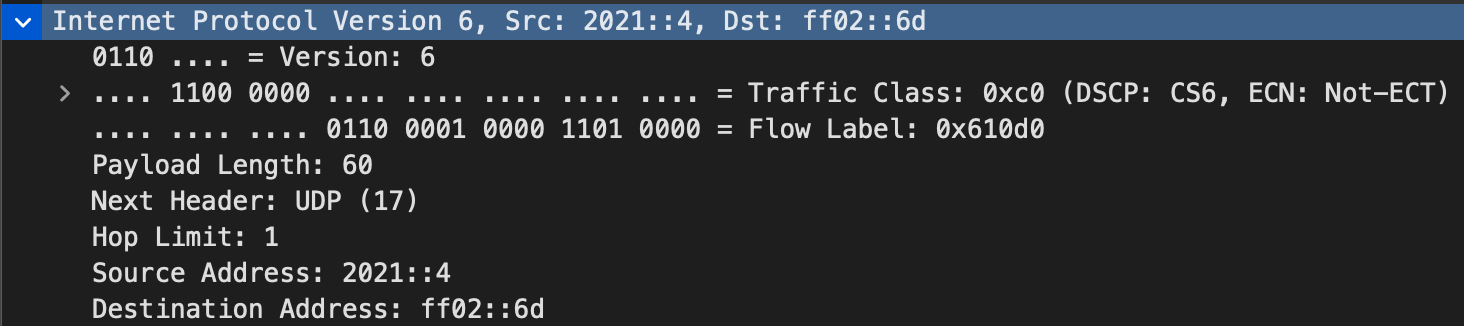
\includegraphics[width=.8\linewidth]{figs/image_1.png}
    \caption{Pacote HELLO}
    \label{fig:1}
\end{figure}

\section{Pergunta 2} \label{ex2}

Dado que neste cenário todos os nodes estão ligados ao mesmo switch, isto significa que eles conseguem se ver entre todos.
Para simular as diferentes configurações, temos que filtrar o tráfego que "supostamente" não deve existir.

Por exemplo, analisando a tipologia em linha, no PC1 temos que filtrar todo o tráfego para o PC3 e PC4, que nesta configuração,
o PC1 não devia conseguir ver.

\begin{figure}[H]
    \centering
    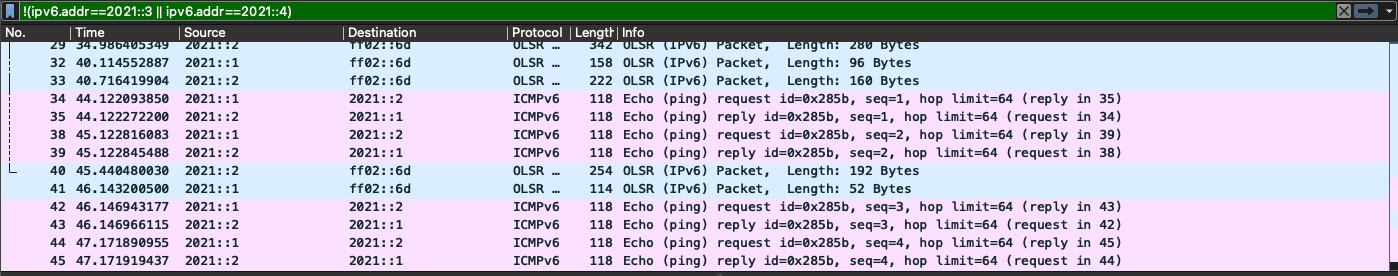
\includegraphics[width=.8\linewidth]{figs/image_2.png}
    \caption{Análise do tráfego no PC1 com filtros}
    \label{fig:2}
\end{figure}

Após aplicar os filtros correspondentes, podemos analisar a largura de banda utilizada por cada node.
Os dados a considerar são apenas das mensagens de controlo, (OLSR v1), pois estas são automáticas e constantes.
Se considerássemos os pings efetuados, os dados estariam errados pois os pings não são constantes e dependem do que o utilizador fez. 

\begin{table}
\begin{center}
    \Large{
    \begin{tabular}{ | c | c| c | c | c |} 
    \hline
    Bandwidth (bits/s) & PC1 & PC2 & PC3 & PC4 \\ 
    \hline
    Linha & 442 & 696 & 721 & 435\\ 
    \hline
    Estrela & 467 & 693 & 451 & 436\\
    \hline
    \end{tabular}
    }
\end{center}
\caption{Bandwidth em linha e em estrela}
\label{tab:1}
\end{table}

No caso da tipologia em linha, quer o PC1 quer o PC4 só vêm um node, PC2 e PC3 respetivamente. Já o PC2 e PC3 vêm dois nodes cada.
Deste modo, é de esperar que o PC2 e PC3 gerem mais tráfego que o PC1 e PC2, dado que vêm mais nodes. Isto é facilmente visível na tabela,
onde o PC2 e PC3 geram aproximadamente mais 50\% de tráfego com mensagens de controlo.

No caso da tipologia em estrela, o PC2 é vizinho de todos os outros PCs, enquanto os que outros PCs apenas têm um vizinho.
Deste modo, é de esperar que largura de banda usada pelo PC2 seja superior aos outros computadores, o que se verifica nos dados obtidos.


\section{Pergunta 3} \label{ex3}

Para efetuar o teste, procedemos à mudança de tipologia nos PCs e reiniciámos o protocolo OLSR após a reconfiguração.
O instante t=0 na captura do \textit{Wireshark} corresponde ao momento em que o protocolo foi iniciado no último PC (PC1).
Imediatamente a seguir, executamos constantemente o comando h1 ping6 2021::4 para enviar um ping entre o PC1 e o PC2.
Este pedido não foi no entanto capturado pelo Wireshark, dado que o nesse momento o PC1 ainda não conhecia a existência do PC4.
Após 32 segundos, o PC1 finalmente já tinha informação relativamente ao PC4 e ao caminho e os pings passaram a ser lidos pelo \textit{Wireshark}.

\begin{figure}[H]
    \centering
    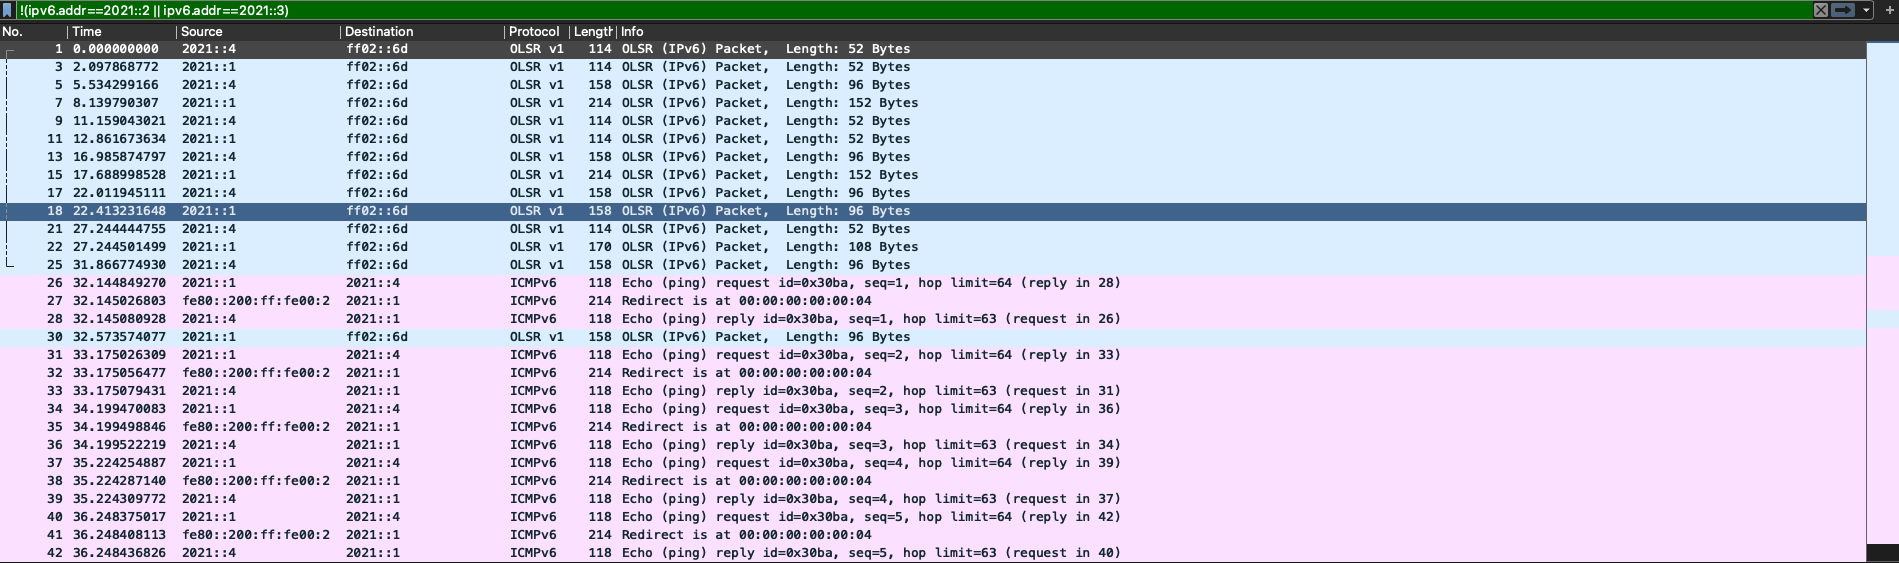
\includegraphics[width=.9\linewidth]{figs/image_3.png}
    \caption{Ping do PC1 para PC4 após mudança de tipologia}
    \label{fig:3}
\end{figure}

Entre o primeiro ping e o a primeira resposta temos um intervalo de aproximadamente 32 segundos.
Este tempo faz sentido dado que a soma do tempo do um pacote HELLO (10s) e TC (6s) é de 16 segundos.
Este processo tem que ser efetuado duas vezes, do PC4 para o 2 e depois do PC2 para o PC1, daí os 32 segundos.

\clearpage

\section{Pergunta 4} \label{ex4}

A resposta a esta pergunta está parcialmente presente na secção \ref{ex2}.

A função dos MPR é de otimização da transmissão dos pacotes HELLO e TC dentro da rede MANET.
Deste modo, minimizamos o tráfego desnecessário na rede e diminuímos a largura de banda necessária \cite{mpr}.

Na tipologia de linha, os MPR serão o PC2, escolhido pelo PC1 e PC3, e o PC3, escolhido pelo PC2 e PC4, que são os PCs que permitem comunicação 2-hop aos PCs que os escolheram.
Como observamos na tabela \ref{tab:1}, os PC2 e PC3 geram mais tráfego, que é um bom indicador do comportamento de MPRs.

\begin{figure}[H]
    \centering
    \begin{subfigure}{.5\textwidth}
      \centering
      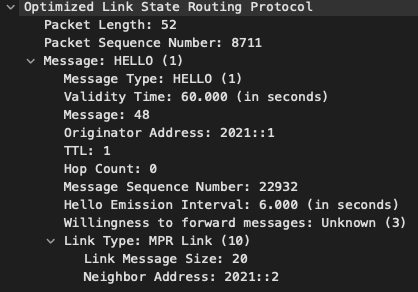
\includegraphics[width=.9\linewidth]{figs/image_4.png}
      \caption{MPR do PC1}
      \label{fig:4_1}
    \end{subfigure}%
    \begin{subfigure}{.5\textwidth}
      \centering
      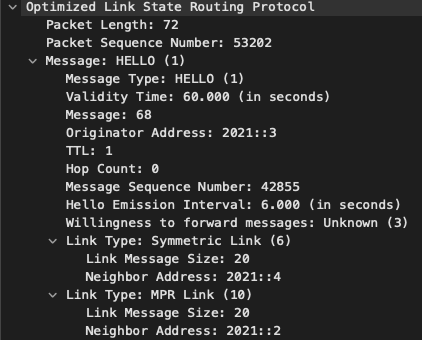
\includegraphics[width=.9\linewidth]{figs/image_6.png}
      \caption{MPR do PC3}
      \label{fig:4_2}
    \end{subfigure}
    \caption{PC2 como MPR}
    \label{fig:4}
\end{figure}

Na figura \ref{fig:4_1}, o PC1 escolhe o PC2 como o seu MPR.
Na figura \ref{fig:4_2}, o PC3 tem o PC2 como um \textit{MPR Link} e o PC4 como um \textit{Symmetric Link}.

\begin{figure}[H]
    \centering
    \begin{subfigure}{.5\textwidth}
      \centering
      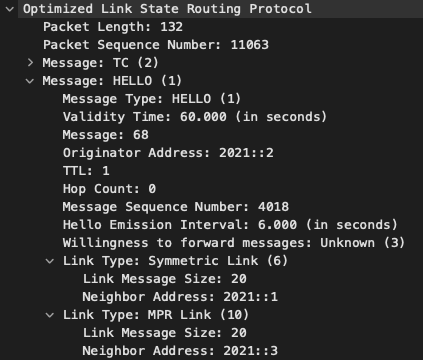
\includegraphics[width=.9\linewidth]{figs/image_5.png}
      \caption{MPR do PC2}
      \label{fig:5_1}
    \end{subfigure}%
    \begin{subfigure}{.5\textwidth}
      \centering
      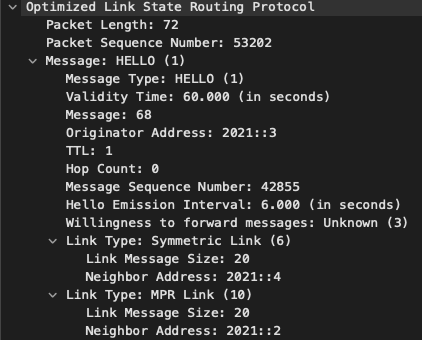
\includegraphics[width=.9\linewidth]{figs/image_6.png}
      \caption{MPR do PC4}
      \label{fig:5_2}
    \end{subfigure}
    \caption{PC3 como MPR}
    \label{fig:5}
\end{figure}

Uma situação semelhante se pode verificar quando ao PC3.
Na figura \ref{fig:4_1}, o PC2 escolhe o PC3 como o seu MPR.
Na figura \ref{fig:4_2}, o PC4 tem o PC3 como um \textit{MPR Link} e o PC2 como um \textit{Symmetric Link}.


Na tipologia em estrela, o PC2 será escolhido por todos os PCs como MPR dado que é o centro da configuração em Estrela.
O PC2 é o CP que permite comunicações 2-hop para todos.
Enquanto que o PC2 vê todos os PCs, estes só vêm o PC2.

\begin{figure}[H]
    \centering
    \begin{subfigure}{.33\textwidth}
        \centering
        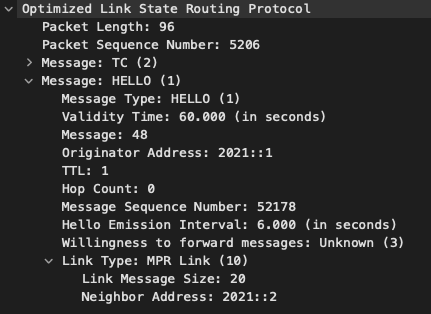
\includegraphics[width=.95\linewidth]{figs/image_8.png}
        \caption{MPR do PC1}
        \label{fig:6_1}
    \end{subfigure}%
    \begin{subfigure}{.33\textwidth}
        \centering
        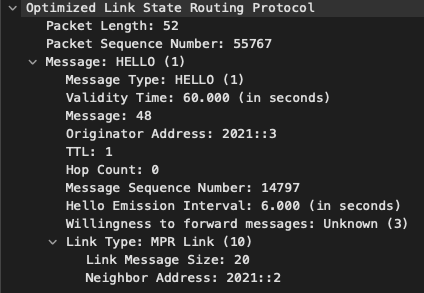
\includegraphics[width=.95\linewidth]{figs/image_9.png}
        \caption{MPR do PC3}
        \label{fig:6_2}
    \end{subfigure}
    \begin{subfigure}{.33\textwidth}
        \centering
        \includegraphics[width=.95\linewidth]{figs/image_10.png}
        \caption{MPR do PC4}
        \label{fig:6_}
    \end{subfigure}
    \caption{PC2 como MPR}
    \label{fig:6}
\end{figure}

Como podemos observar na figura \ref{fig:6}, todos os PCs escolhem o PC2 como o seu MPR.

\begin{figure}[H]
    \centering
    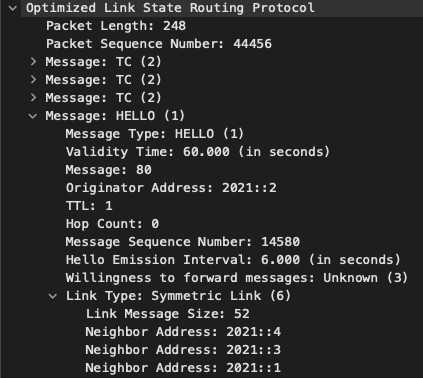
\includegraphics[width=.8\linewidth]{figs/image_11.png}
    \caption{Links do PC2}
    \label{fig:7}
\end{figure}

Dado que o PC2 consegue comunicar com todos os PCs em one-hop, não precisa de MPR.
Desse modo, assume todos os links que tem com os restantes PCs como \textit{Symmetric Links}.


\section{Pergunta 5} \label{ex5}

\begin{figure}[H]
    \centering
    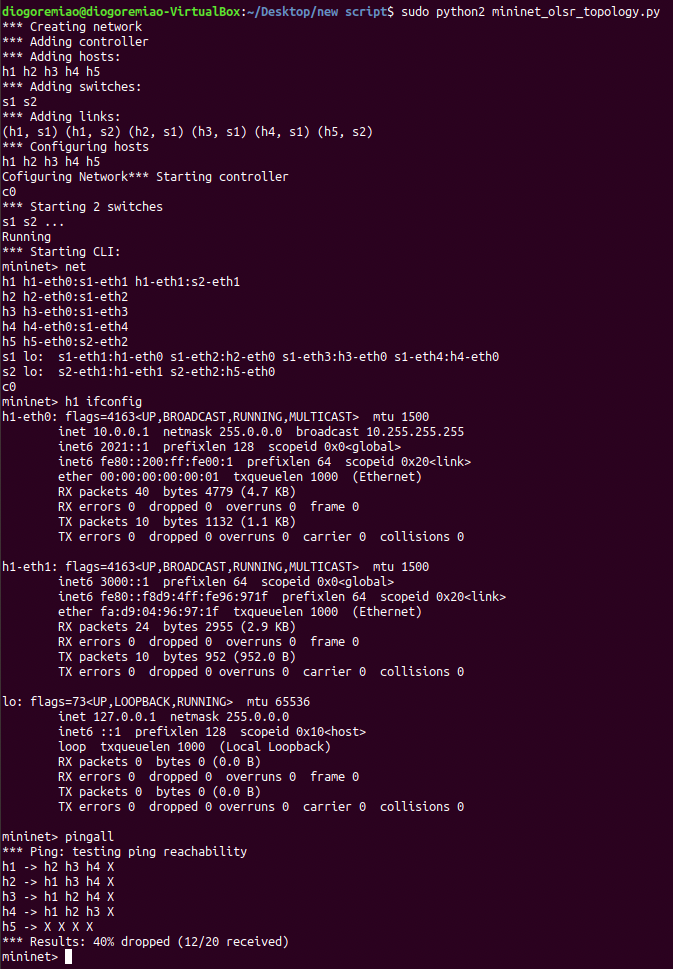
\includegraphics[width=.8\linewidth]{figs/image_12.png}
    \caption{Output do script Python}
    \label{fig:8}
\end{figure}


O Mininet oferece uma command-line interface que nos permite correr comandos específicos de cada host \cite{mininet}.
No entanto, para podermos utilizar o comando é preciso um \textit{Mininet Object}, especificando a classe topo do OLSR e o controlador OVS.
Desta forma, conseguimos agora resolver os diferentes hosts acedendo a este objeto e podemos correr agora os comandos indicados para cada host (Anexo \ref{py_script}).

Na figura \ref{fig:8} podemos observar que correndo por exemplo \textit{ifconfig} no host 1, a interface h1-eth0 está configurada para IPv6 como indicado.
O comando \textit{net} dá como output as diferentes interfaces que foram configuradas.
Finalmente, correndo \textit{Pingall} verificamos a conexão entre todos os hosts, garantindo que os comandos foram de facto executados para cada hosts,
e o sistema funcional.

\section{Pergunta 6} \label{ex6}

Mais uma vez, o novo \textit{Mininet Object} prova-se útil, dado que nos permite aceder diretamente à network e aos diferentes hosts.
Deste modo, usando mais uma vez a CLI do Mininet, podemos fazer uso da API Python disponibilizada pelo Mininet para fazer as alterações necessárias.
Para dizer ao Mininet que se está a tentar correr um comando python, tem que se por o prefixo \textit{py} antes de todos os comandos.

O comando \textit{net.addHost('h6')} permite adicionar mais um host à rede, neste caso o h6.

De seguida é preciso ligar o host ao switch, utilizando o comando \textit{net.addLink(net.get('s1'), net.get('h6'))}.

Depois deste passo, é preciso ligar a interface no switch, que é feito automaticamente na classe \textit{topo} mas não na classe \textit{net}.
Isto é feito com o comando \textit{net.get('s1').attach('s1-eth0')} na classe \textit{node}.

Por fim, é atribuído um IP ao novo host com o comando \textit{net.get('h6').setIP('10.0.0.6')}, mais um vez na classe \textit{node}.

\begin{figure}[H]
    \centering
    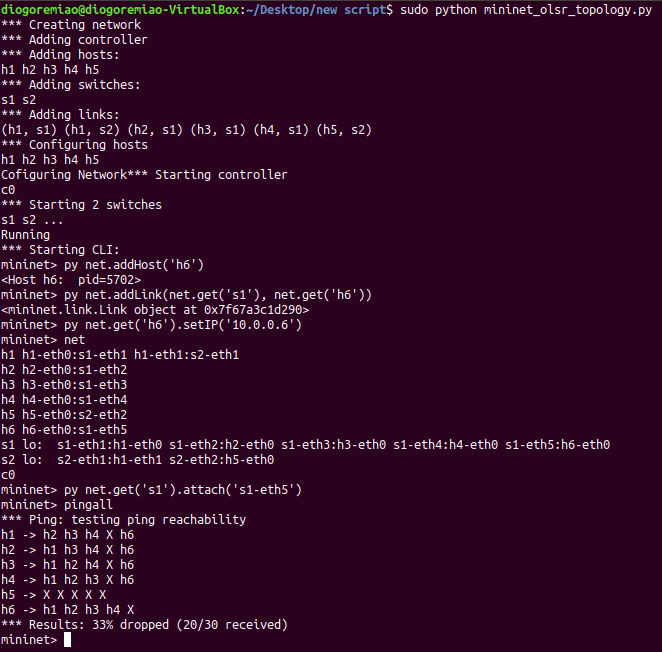
\includegraphics[width=.8\linewidth]{figs/image_13.png}
    \caption{Uso da API Python do Mininet para adicionar um novo host}
    \label{fig:9}
\end{figure}

